\documentclass[a4paper,10pt]{article}
\usepackage{tabularx}
\usepackage{multirow}
\usepackage{graphicx}
\usepackage{float}
\usepackage{wrapfig}
\usepackage[left=0.75in,top=0.55in,right=0.75in,bottom=0.7in]{geometry}
\usepackage{hyperref}
\usepackage[backend=bibtex]{biblatex}
\usepackage[export]{adjustbox}
\usepackage[english]{babel}


\title{Rube Goldberg Machine   \\ Serve water in Style!!}
\author{The Blitz Exterminators}
\addbibresource{bib1}
\begin{document}
\maketitle
\section*{Group Details}
We try to automate every task possible.And we exterminate our problems as they come our way,crushing them like bugs. We are \textbf{The Blitz Exterminators}.
\begin{center}
\begin{tabular}{ |c|c|c|}
\hline
\textbf{Group Name} & \textbf{Roll No.} & \textbf{Name} \\
\hline
\multirow{3}{*}{Blitz Exterminators}& 140050003 & Harshal\\
& 140100011 & Tanmay \\
& 140100090 & Navneet\\
\hline
\end{tabular}
\end{center}
\hfill \break
\begin{center}
\section*{Our Design}
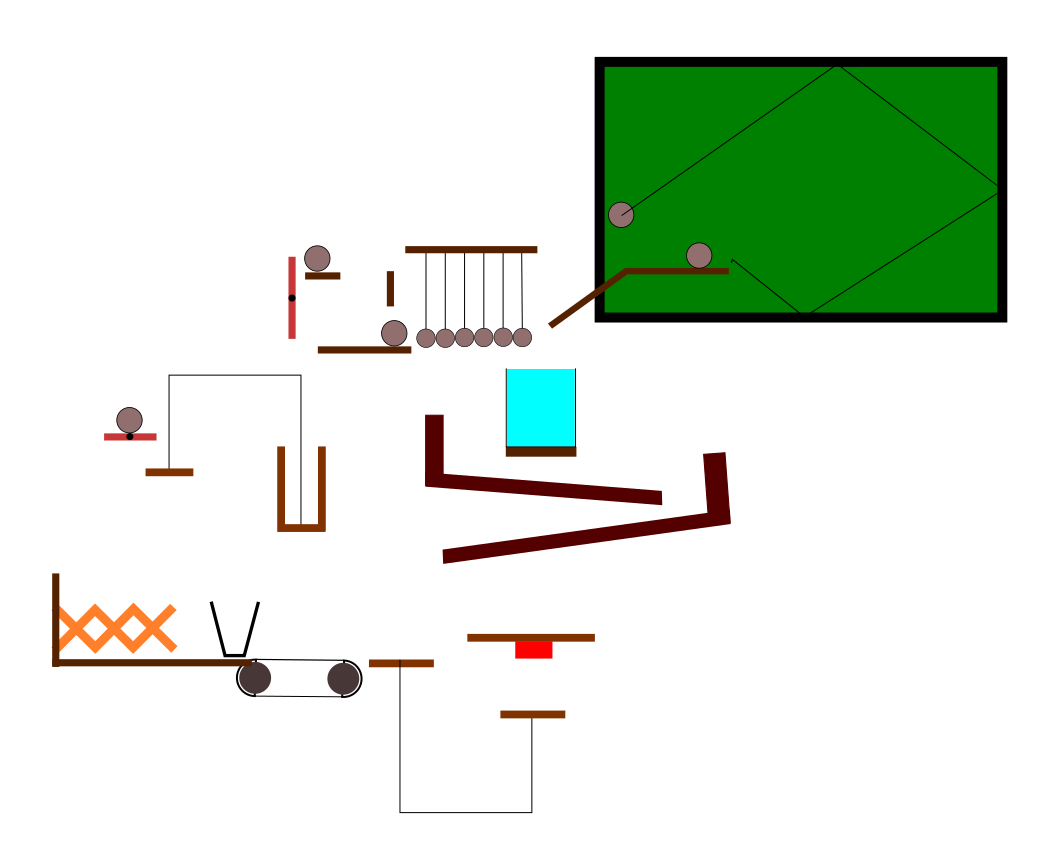
\includegraphics[width=0.75\textwidth]{img}\nocite{inkscape}
\end{center}
\newpage
\section*{Our Motivation}
\begin{wrapfigure}{l}{0.5\textwidth}

\begin{center}
\vspace{-20pt}
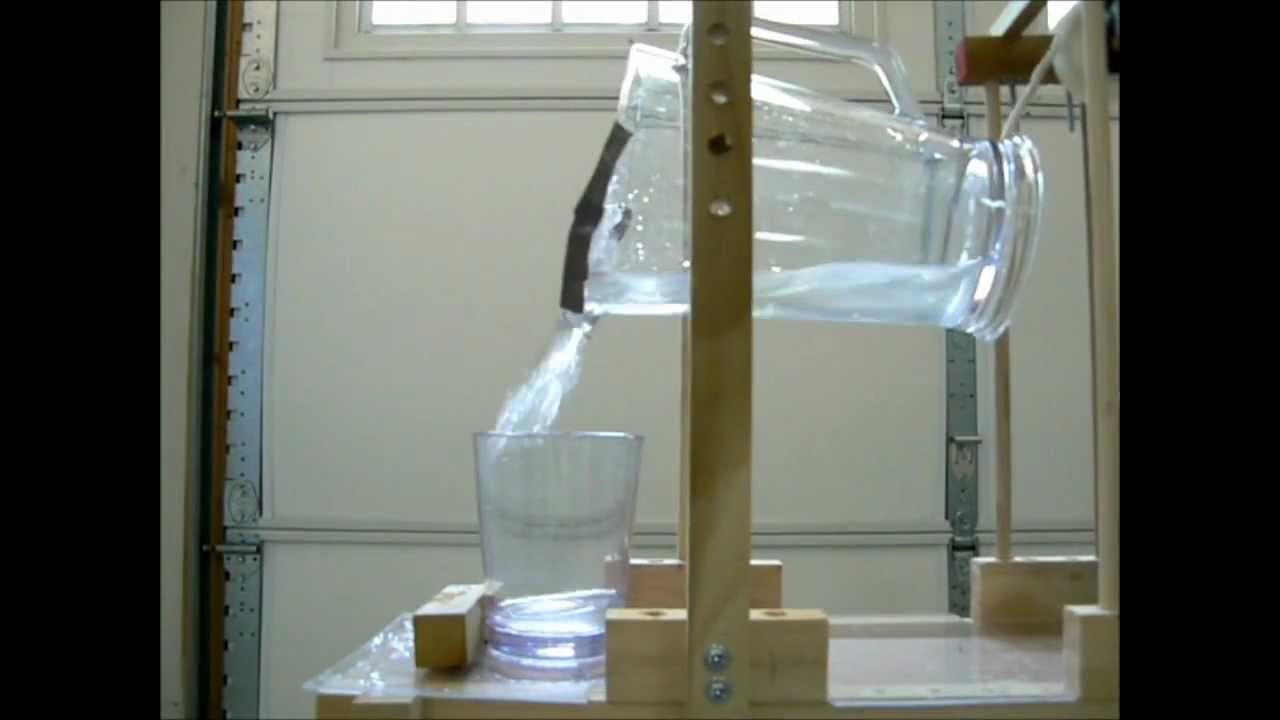
\includegraphics[width=0.4\textwidth]{img2}

\caption{Our Goal from Machine}\cite{Youtube}
\end{center}
\end{wrapfigure}
\hfill \break Whenever we go home while studying especially, we don't like water at our table but we do like having our Mother get some water for us. The worst part is refusal from Mother. So we are designing a Rube Goldberg Machine to achieve this task. Fundamentally, this Machine transfers water from one container to another container which is delivered to our position. It has the most complications we could think of to show off our geeky attitude. After all, we should love science to be in IITB, right?
\\ \\

\section*{Introduction}
This Rube Goldberg Machine is a clssic piece of physics. The Water Server as we like to call performs a really simple task just like any other Rube Goldberg Machine. The goal of this machine is to transfer water from one container to other one and then deliver it using conveyor belt to the user. It is pretty much concise but has a flavour of geekiness added along with art of imagination.
\section*{Equations and principles used}

	\begin{enumerate}
	\item 	Archimedes Principle
	\item 	Theory of Gravitation
	\item   Newton's Laws of Motion
	\end{enumerate}

\section*{Parts}
We can classify the elements basically into 3 categories based on their functions althought the parts are obviously intertwined with each other, it is really neccessary that the parts function together
\subsection*{Part 1: Initialization and setting up}
\begin{wrapfigure}{r}{0.5\textwidth}

\begin{center}
\vspace{-10pt}
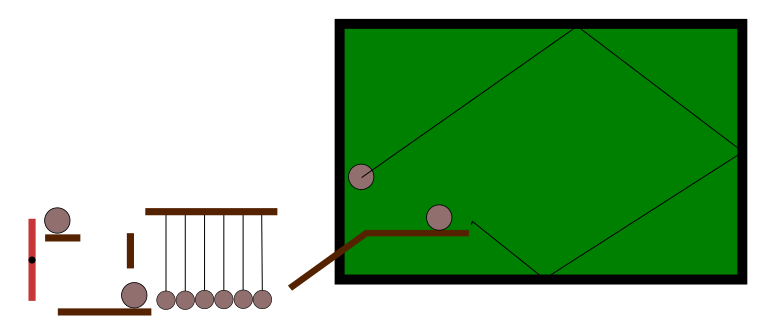
\includegraphics[width=0.4\textwidth]{img_p2}

\caption{Initializing the Motion}
\end{center}
\end{wrapfigure}
\hfill \break The set is initialized by a snooker ball (kinematic object) which bounces off 3 of the 4 sides in a classical way to trigger the motion required. The ball hits another ball on the ramp which in turn hits the Newtons Cradle in the left part. The Newton's Cradle hits another ball which hits another ball above it via a lever.\\ \\ 
\clearpage
\subsection*{Part 3: Spliting the paths}
\begin{wrapfigure}{r}{0.5\textwidth}

\begin{center}
\vspace{-30pt}
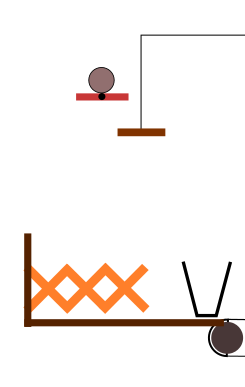
\includegraphics[width=0.2\textwidth]{img_p1}

\caption{Initializing the Motion}
\end{center}
\end{wrapfigure}
\hfill \break The two balls that hit the Newtons Cradle hit the bucket and the platform which is connected to the container using a pulley is pulled upward, pushing the ball to fall on the spring like compressible system. This system pushes the glass on to the conveyor belt.\\ \\
\medskip
\medskip
\hfill \break
\hfill \break\hfill \break
\hfill \break
\hfill \break
\subsection*{Part 3: Final execution}
\begin{wrapfigure}{r}{0.5\textwidth}

\begin{center}
\vspace{-30pt}
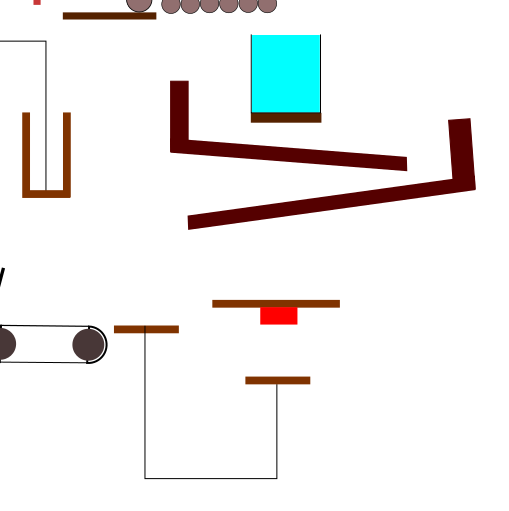
\includegraphics[width=0.3\textwidth]{img_p3}

\caption{Initializing the Motion}
\end{center}
\end{wrapfigure}
\hfill \break The ball that hits Newton's Cradle falls in to water and the water overflows. The water that overflows is collected in the glass that is passed from step 2. It also triggers an alarm and Voila! glass of water is ready.\\ \\
\clearpage
 


 
 \medskip
 
%\begin{thebibliography}{9}
%\bibitem{Youtube} 
%Water Pouring Rube Goldberg Simple Machine Course- TheEpicSpaniardRS,
%\\ \href{https://www.youtube.com/watch?v=fQafL75ud7A}{Link}
%
%\bibitem{inkscape} 
%Inkscape Dcumentation
%\\ \href{https://inkscape.org}{Link}
%
%\bibitem{ShareLatex} 
%Share$\LaTeX$ Tutorials
%\\ \href{https://www.sharelatex.com/learn/Bibliography_management_in_LaTeX}{Link}
%
%\end{thebibliography}

\printbibliography
\nocite{ShareLatex}

\end{document}          
